\chapter {Introduction to Trees}
 A tree is somewhat
similar to a linked list, but, when used properly, can provide very fast
access to specific data elements because data is stored in a sorted
fashion. There are many new terms in this chapter. 

The first section  will familiarize you with the terms and
concepts you will need to understand the algorithms for working with
trees in your programs.

Subsequent sections will help you understand the algorithms
associated with constructing and maintaining a  tree.   It is to your advantage to ensure that you understand the concepts in this chapter before trying to learn about the specific algorithms for binary trees.   Trees are a fundamental data structure in many programming languages and are the base data structure for several other data types including heaps, priority queues,  and search trees.

\section {Simple Rooted Trees}

A tree ADT is similar to a linked list in that it consists of a series
of connected nodes. Unlike a linked list node, a tree node can be
connected to more than two other nodes.

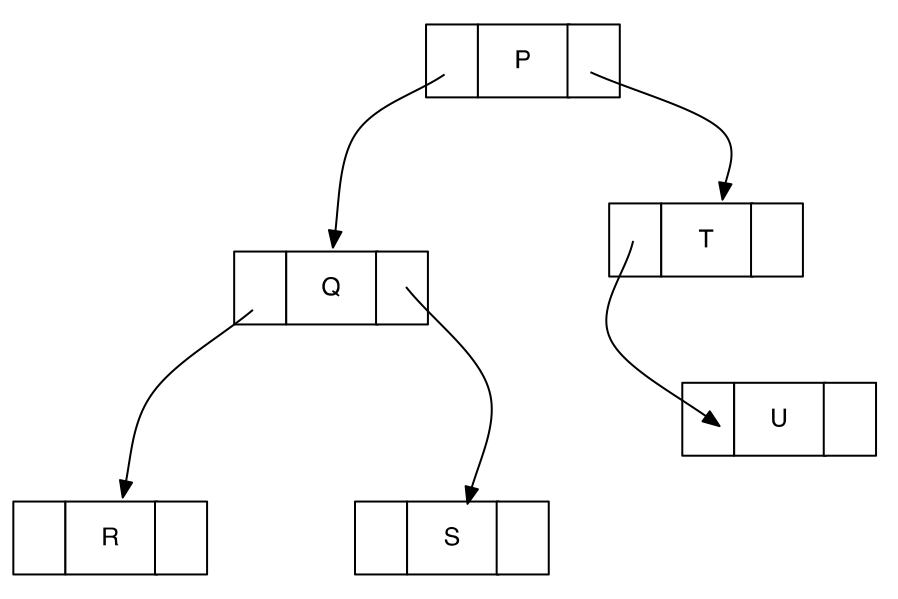
\includegraphics[width=5.80556in]{pictures/image1.png}

Consider the picture above. It shows a tree with six nodes. There are
several terms that you must understand before you can really understand
how a tree ADT works.

\begin{itemize}
\item
  Nodes in trees have relationships to other nodes. We label these
  relationships as \emph{parent}, \emph{child}, \emph{ancestor}.

  \begin{itemize}
  \item
    Node Q in the picture is a child of node P. Node P is the parent of
    nodes Q and T. Node P is the ancestor of node S.
  \item
    Nodes can only have one parent
\end{itemize}
\item
  A tree has a \emph{root node.} In fact a tree can have only one root
  node. The root node has no parent. In the example tree, P is the root
  node.
\item
  Trees have branches. The path between two nodes is called a branch. In
  the example, nodes P and Q have two branches, node T has one branch
  and nodes R, S and U have zero branches.
\item
  Nodes with no branches are known as leaf nodes.
\item
  A tree has a height. The height is the number of nodes in the longest
  path from the root to a leaf. The height of the example tree is 2
  because the longest path is from P to Q to (R or S).  Some algorithms for calculating height count the root node as height one.  For this course we will not count the root node in the height by default.  If the root node is counted it will be explicitly noted.
\item
  Each node in the tree has a level. In the example, nodes Q and T are
  on level 1 because they are children of the root. R, S and U are on
  level 2.
\item
  Trees are recursive: each branch of a tree (each subtree) is also a
  tree.
\end{itemize}
  
  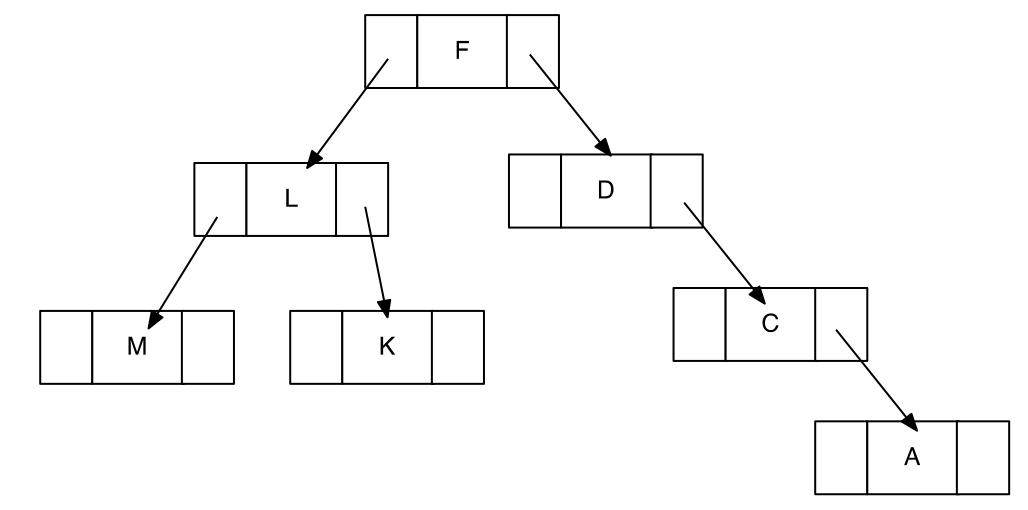
\includegraphics[width=6.00000in]{pictures/image2.png}

Can you answer the following questions about the tree image shown above?  

  How many nodes are in the tree?  (answer 7)

  What is the height of this tree? (answer 3)

  Which node is the root node of the tree? (answer F)

  Which nodes are leaf nodes of the tree? (M, K, A)

  Which node is the parent of node K? (L)

  What is the largest number of branches that any node in this tree has? (2)


 \section {Operations on Trees} 
 \subsection{Tree Insertions}
  When nodes are inserted into a tree, the operation is performed such
  that the nodes are kept in sorted order in the tree. Sorted order can
  be defined any way that the programmer wishes. For example nodes could
  be sorted alphabetically, or they could be sorted by numeric value,
  length, or by some other attribute.
   
   Data entry into a tree is a bit more complicated than it is for linked
  lists. Suppose we were creating a linked list from the following names
  and we wished to keep the list sorted:
  
\begin{itemize}
\item Dopey
\item Sleepy
\item Happy
\item Doc
\item Sneezy
\item Grumpy
\item Bashful
\end{itemize}

We would create the list with the first entry of Dopey and then we'd
insert Sleepy behind it. Happy would get inserted between Dopey and
Sleepy, Doc would be inserted before Dopey, Grumpy would be added after
Dopey and Bashful would be inserted at the head of the list. The
completed list would look something like this:

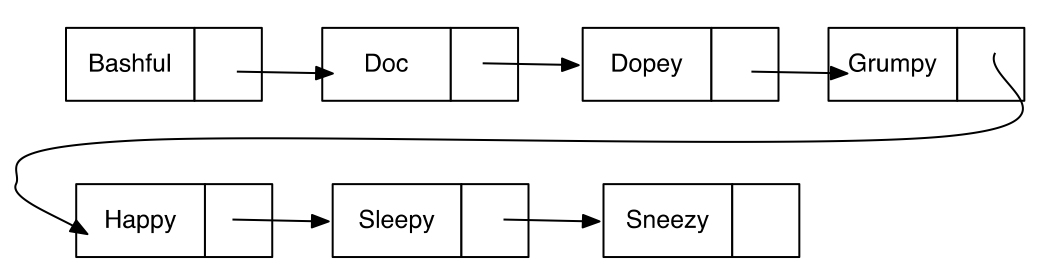
\includegraphics{pictures/image3.png}

However, if we were storing the same data in a tree ADT the
insertion/addition process would be slightly different. Trees use a
compare function to decide if the node to be inserted is larger, or
smaller than the node being compared. Nodes that are larger than the
current node are placed in the right branch, nodes that are smaller than
the current node are placed in the left branch.

So if we started the tree by entering Dopey, the second node, Sleepy,
would be placed in the right branch because Sleepy is `larger'
alphabetically than Dopey. Happy also goes to in the right hand branch
of Dopey, but in the left hand branch of Sleepy because Happy is bigger
than Dopey, but smaller than Sleepy. The finished tree can be seen
below:

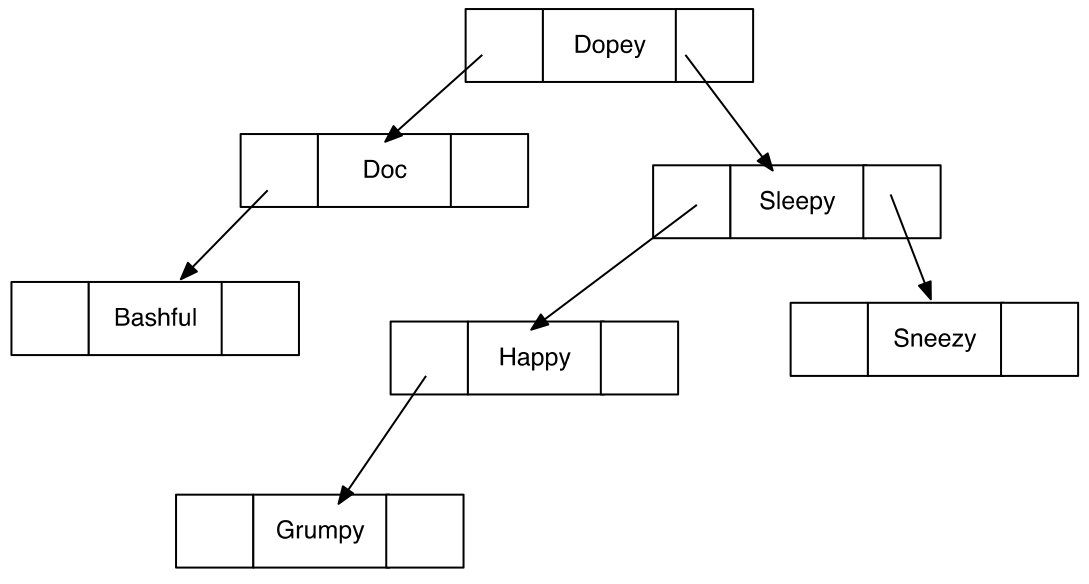
\includegraphics[width=6.00000in]{pictures/image4.png}

\subsection{Removing nodes from a tree}

Because tree nodes can have two children,  the removal of nodes from a tree is more complicated than removing elements from a list.  
Consider the tree shown in the previous section.   If "Doc" were removed from the tree,  the tree could be reconfigured so that Dopey pointed to Bashful and the sorted nature of the tree would not be compromised.

However,  if "Sleepy" were to be removed from the tree, the reconfiguration is much more challenging.  Should  Dopey point to Happy or to Sneezy?  What happens to the other node?    Many tree libraries do not actually delete an element from a tree on removal,  instead the library marks the element "inactive".   It holds its place in the tree, but cannot be returned on searches and cannot be updated.  

We will discuss removing nodes from trees more in subsequent chapters.

\subsection{Tree Traversal}

Nodes in the trees are accessed by traversing the tree. Traversal is
simply a process of walking through the tree by using the pointers that
connect nodes to move from one node to the next. Tree traversal always
starts with the root node of the tree.   An \textbf{iterator} can be used to traverse a tree if the Tree ADT comes with an iterator function.

Imagine that your task was to print all of the values of the nodes in
the tree. What order would they be printed in if you started at the root
node? The answer to that question depends on when you printed each node
and which branches of the tree you followed first. The different
patterns of walking through the tree are traversal schemes.  Two common
schemes are in-order traversal and pre-order traversal.  Both of these traversal algorithms are recursive.



\subsubsection{Pre-order traversal}

Another common traversal technique is Pre-order traversal. The general
idea is the same but the algorithm changes slightly to process the root
node first, before any subtrees are processed. The general algorithm is:

process current node

process left subtree

process right subtree


The pre-order traversal of the tree example shown in section YYYYY is
 Dopey, Doc, Bashful, Sleepy, Happy, Grumpy, Sneezy.
 
 \begin{lstlisting}[showspaces=false, language=make]
 We start at the root (the current node) and print it - Dopey.
   Recurse on the left subtree - printing Doc
         Recurse on Doc's left subtree- printing Bashful
            Bashful has no left subtree
            Bashful has no right subtree
            Return
         Doc has no right subtree
      Recurse on the right subtree - printing Sleepy
         Recurse on Sleepy's left subtree - printing Happy
            Recurse on Happy's left subtree printing Grumpy
               Grumpy has no left subtree
               Grumpy has no right subtree
               return
             Happy has no right subtree
             Return
           Recurse on Sleepy's right subtree printing Sneezy
                 Sneezy has no left subtree
                 Sneezy has no right subtree
                 Return
\end{lstlisting}		     		
				
\subsubsection{In-order traversal}

An in-order traversal visits each node in sort order and processes the
node as it is visited. For example, if the nodes in the example tree
were traversed in order, and the processing action was to print the
value, the result would be an alphabetized list of names.

To conduct an in-order traversal, the algorithm must move to the
smallest value in the tree (which will be the left most leaf), process
that leaf, move to its parent, process the parent, move to the right
branch and repeat.

For each tree (and subtree) the algorithm is:

\begin{itemize}
\item
  process left subtree
\item
  process root
\item
  process right subtree
\end{itemize}

The key difference between pre-order and in-order traversal is when the root node is processed.  The in-order traversal for the example tree  is  shown below:

\begin {lstlisting}
Start at the root but do not process it
Recurse to process the left subtree.
	This means we must move to Doc but do not process it because it is the root
		Recurse to process the left subtree
			This means we must move to Bashful but do not process it
			Bashful has no left subtree
			process the root and print Bashful
			Bashful has no right subtree so we return
		Process the root and print Doc
		Doc has no right subtree so we return
	process the root and print Dopey
	Recurse to Process the right subtree
		This means we must move to Sleepy
			Recurse to process the left subtree
			This means we must move to Happy
			Recurse to process the left subtree
				This means we must move to Grumpy
				Grumpy has no left subtree
				process the root and print Grumpy
				Grumpy has no right subtree so we return
			process the root and print Happy
			Happy has no right subtree so we return
		Process the root and print Sleepy
		Recurse to Process the right subtree
			This means we move to Sneezy
			Sneezy has no left subtree
			process the root and print Sneezy
			Sneezy has no right subtree so we return
			
			done.
\end{lstlisting}




